\chapter{Correctness}
\paragraph{}In this section, we show that, once topology changes cease, the algorithm eventually terminates with each connected component being leader-oriented. As a result, the lidu variables satisfy the conditions of the leader election problem.
\paragraph{}We first show, in Section 4.1, an important relationship between the final commu- nication topology and the forming and N variables of the nodes. The rest of the proof uses a number of invariants, denoted as “Properties”, which are shown to hold in ev- ery configuration of every execution; each one is proved (separately) by induction on the configurations occurring in an execution. In Section 4.2, we introduce some def- initions and basic facts regarding the information about nodes’ heights that appears in the system, either in nodes’ height arrays or in messages in transit. In Section 4.3, we bound, in Lemma 3, the number of elections that can occur after the last topology change; this result relies on the fact, shown in Lemma 2, that once a node u adopts a leader that was elected after the last topology change, u never becomes a sink again. Then in Section 4.4, we bound, in Lemma 4, the number of new reference levels that are started after the last topology change; the proof of this result relies on several additional properties. Section 4.5 is devoted to showing, in Lemmas 5, 6, and 7, that eventually there are no messages in transit and every node has an accurate view of its neighbors’ heights. All the pieces are put together in Theorem 1 of Section 4.6 to show that eventually we have a leader-oriented connected component; a couple of additional properties are needed for this result.
\paragraph{}Throughout the proof, consider an arbitrary execution of the algorithm in which the last topology change event occurs at some global time tLTC , and consider any connected component of the final topology.
\section{Channels and Neighbors}
\paragraph{}Because of the lack of coordination between the topology change events for the two channels going between nodes u and v in the two directions, u and v do not neces-sarily have consistent views of their local neighborhoods in Gchan , even after the last topology change. For instance, it is possible that v is in Nu but u is not in Nv forever after the last topology change. Suppose the channel from u to v remains Up from some time t onwards, so that v remains in Nu from time t onwards. However, suppose that the channel from v to u fluctuates several times after time t, eventually stabilizing to being Up (cf. Fig. 5). Every time the channel to u goes down, u is removed from v’s forming and N sets. Every time the channel to u comes up, v adds u to formingv and sends its height in an Update message to u. When u gets the message from v, it updates the entry for v in its height array, but does not send its own height back to v. As long as u’s height does not change, u does not send its height to v. Thus v is never able to move u from formingv into Nv.
\begin{figure}[h]
	\centering
	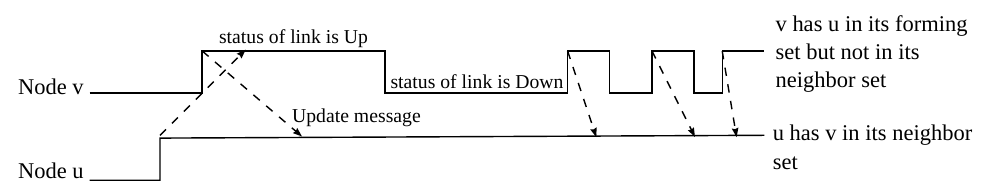
\includegraphics[width=1\linewidth]{fig_1}
	\caption[The status of the channel from u to v remains Up, but the status of the channel from v to u fluctuates.]{The status of the channel from u to v remains Up, but the status of the channel from v to u fluctuates.}
	\label{fig:fig1}
\end{figure}
\paragraph{}However, we are assured by Lemma 1 below that after time tLTC , $N_u \cup forming_u$ does not change for any node u. Furthermore, a node u always sends Update messages to all nodes in $N_u \cup forming_u$ , which constitutes all the outgoing channels of u.
\paragraph{Lemma 1}After time $t_{LTC}$ , $N_u \cup forming_u$ does not change for any node u.
\subparagraph{Proof}When ChannelDownuv occurs, u removes v from both its Nu and formingu variables. When ChannelUpuv occurs, u adds v to its formingu variable and sends an Update message to v. When u receives an Update message from a node v, the only possible change to the Nu and formingu variables is that v is moved from formingu to Nu , which does not change $N_u \cup forming_u$.
\subparagraph{}tT LC is the latest among all the times at which either a ChannelDown, or a Chan- nelUp occurs. After this time, the only change to the N set or the forming set must be due to receipt of an Update message, causing lines 2 and 3 of Figure 2 to be executed. Thus the only change to the N set or the forming set is that a node which is removed from the forming set is added to the N set. This does not affect $N \cup forming$.
\section{Height Tokens and Their Properties}
\paragraph{}Since a node makes algorithm decisions based solely on comparisons of its neigh- boring nodes’ height tuples, we first present several important properties of the tuple contents. Define h to be a height token for node u in a configuration if h is in an Update message in transit from u, or h is the entry for u in the height array of any node. Let LP(h) be the leader pair of h, RL(h) the reference level (triple) of h, $\delta(h)$ the $\delta$ value of h, lts(h) the absolute value of the (nonpositive) leader timestamp (component nlts) of h, and $\tau (h)$ the $\tau$ value of h.
\paragraph{}Given a configuration in which Channel(u, v) has status Up and $u \in N_v$ , the (u, v) height sequence is defined as the sequence of height tokens $h0, h1, ... , hm$, where h0 is u’s height, hm is v’s view of u’s height, and $h1 , . . . , h_{m-1}$ is the sequence of height to- kens in the Update messages in transit from u to v. If the status of Channel(u, v) is Up but $u \not\in N_v$ , then the (u, v) height sequence is defined similarly except that $h1 , . . . , h_m$ is the sequence of height tokens in the Update messages in transit from u to v; in these cases, v does not have an entry for u in its height array. If Channel(u, v) is Down, the (u, v) height sequence is undefined.
\paragraph{Property A} If h is a height token for a node u in the (u, v) height sequence, then:
\begin{enumerate}
	\item $lts(h) \leq \mathcal{T} _u$ and $\tau (h) \leq \mathcal{T} _u$
	\item If h is in v’s height array then $lts(h) \leq \mathcal{T} _v$ and $\tau (h) \leq \mathcal{T} _v$ .
\end{enumerate}

\paragraph{Proof}By induction on the configurations in the execution.
\paragraph{}\textit{Basis:} In the initial configuration $C_0$ , all the leader timestamps and $\tau$ values are 0 and $\mathcal{T} \geq 0$ for all nodes v.
\paragraph{}\textit{Inductive Hypothesis:} Suppose the property is true in configuration Ci-1 and show it remains true in configuration Ci . Since the property is true in $C_{i-1}$ , for every height token h in the (u, v) height sequence, we have:
\begin{enumerate} [label=(\roman*)]
	\item $lts(h) \leq \mathcal{T} _u(Ci-1)$ and $\tau (h) \leq \mathcal{T} _u(C_{i-1})$
	\item If h is in v’s height array then lts(h) $\leq$ $\mathcal{T} _v(C_{i-1})$ and $\tau$ (h) $\leq$ $\mathcal{T} _v (C_{i-1})$
\end{enumerate}
\paragraph{}\textit{Inductive Step:} If h is a preexisting height token during event ei (the event immediately preceding $C_i$ ), then by the inductive hypothesis and the increasing property of Tu , it follows that $lts(h) \leq \mathcal{T} _u (C_i )$ and $\tau (h) \leq Tu (Ci )$. If, on the other hand, h is created during event ei , then any new values of lts and $\tau$ generated by u are equal to Tu (Ci ) and, thus, the property remains true.
\paragraph{}If h is a height token for node u at some other node v, then h was either present at v during $C_{i-1}$ or was received at v during event ei , immediately preceding Ci . In the first case, by the inductive hypothesis and the increasing property of Tv , it follows that $lts(h) \leq Tv (Ci )$ and $\tau (h) \leq Tv (C_i )$. In the second case, there exists a message through which v received h from u during event ei . Since T preserves causality, by the definition of the happens before relation, it follows that the creation of either $\tau (h)$ or $lts(h)$ preceded the receipt of the message by v. Therefore, in configuration Ci it remains true that $lts(h) \leq Tv (Ci )$ and $\tau (h) \leq Tv (Ci )$.
\paragraph{}Property B, given below, states some important facts about height sequences. If the channel’s status is Up and m = 1, meaning that no messages are in transit from u to v, then Part (1) of Property B indicates that v has an accurate view of u’s height. If there are Update messages in transit, then the most recent one sent has accurate in- formation. Part (2) of Property B implies that leader pairs are taken on in decreasing order. Part (3) of Property B implies that reference levels are taken on in increasing order with respect to the same leader pair. Note that Property B only holds if m > 0.
\paragraph{Property B:}Let h0 , h1 , . . . , hm be the (u, v) height sequence for any Channel(u, v) whose status is Up. Then the following are true if m > 0:
\begin{enumerate}
	\item $h_0 = h_1$.
	\item For all l, $0 \leq l < m, LP(hl ) \leq LP(h_l+1 )$.
	\item For all l, $0 \leq l < m, if LP(hl ) = LP(hl+1 )$, then $RL(hl ) \geq RL(hl+1 )$.
\end{enumerate}
\paragraph{Proof}The proof is by induction on the execution.
\subparagraph{}Initially in C0 , Channel(u, v) is either Up or Down. If Channel(u, v) is Down, then the (u, v) height sequence is undefined. If Channel(u, v) is Up, then the definition of initial configurations states that no messages are in transit and v has an accurate view of u’s height, that is, m = 1 and h0 = h1 .
\subparagraph{}Suppose the property is true in configuration Ci-1 and show it is still true in configuration Ci .
\subparagraph{}Suppose event ei is ChannelDownuv. Then the (u, v) height sequence is not de- fined in Ci .
\subparagraph{}Suppose event ei is ChannelUpuv. By the assumption that the channel up/down events for a given channel alternate, the state of the channel in Ci-1 is Down and there are no messages in transit. Thus in Ci the (u, v) height sequence is h, h, where h is the height of u in Ci , which is stored in u’s height array and is in the Update message that u sends to v. Clearly this height sequence satisfies the three conditions.
\subparagraph{}Suppose event ei is the receipt by v of an Update message from u. In one case, the (u, v) height sequence changes by dropping the last element, if the oldest message in transit takes the place of v’s view of u’s height. In the other case, the (u, v) height sequence does not change if the receipt causes v to record u’s height and add u to Nv . In both cases, the three conditions still hold.
\subparagraph{}Suppose event ei is the receipt by u of an Update message from node w or is a ChannelDown event for a channel to some node other than v. If u does not change its height, then there is no change affecting the property.
\subparagraph{}Suppose u changes its height from h'0 to h.
\subparagraph{}Let the (u, v) height sequence in Ci-1 be h'0 , h'1 , . . . , h'm . By the inductive hypothesis, h'0 = h'1 . By the code, the (u, v) height sequence in Ci is h, h, h'1 , . . . , h'm . In each case we just have to show that h has the proper relationship to h'1 , which equals h'0 .
\subparagraph{}Case 1: ei calls REFLECT R EF L EVEL: All of u’s neighbors are viewed as having the same LP as u, having reference level (t, p, 0) for some t and p, and having a larger height than u.
\subparagraph{}Since u is a sink during the step, RL(h'0 ) $\leq$ (t, p, 0). Since RL(h) = (t, p, 1), and the old and new LP are the same, the property holds.
\subparagraph{}Case 2: ei calls ELECT S ELF: By Property A, lts in LP(h'0 ) is less than or equal to Tu' in configuration Ci-1 . The new leader pair has lts Tu in configuration Ci , which is greater than Tu' . So LP(h) $\leq$ LP(h'0 ).
\subparagraph{}Case 3: ei calls START N EW R EF L EVEL: By Property A, the $\tau$ value in RL(h'0 ) is less than or equal to Tu' at configuration Ci-1 . The new reference level has $\tau$ value Tu at configuration Ci , which is greater than Tu' and the LP is unchanged. So LP(h) = LP(h'0 ) and RL(h) $\geq$ RL(h'0 ).
\subparagraph{}Case 4: ei calls PROPAGATE L ARGEST R EF L EVEL: All neighbors of u are viewed as having the same LP as u, but with different RL's among themselves, and as having larger heights than u. By the code, u takes on the largest neighboring RL, which is at Case 4: ei calls PROPAGATE L ARGEST R EF L EVEL: All neighbors of u are viewed as having the same LP as u, but with different RL’s among themselves, and as having larger heights than u. By the code, u takes on the largest neighboring RL, which is at least as large as u’s old RL, since u is a sink. The LP is unchanged. So LP(h) = LP(h'0 ) and RL(h) $\geq$ RL(h'0 ).
\subparagraph{}Case 5: ei calls ADOPT LPI F P RIORITY: By the code, the new LP is smaller than the previous, so LP(h) < LP(h'0 ).
\section{Bounding the Number of Elections}
\paragraph{}In this subsection, we show that every node elects itself at most a finite number of times after the last topology change.
\paragraph{}Define the following with respect to any configuration in the execution. For LP (-s, l), where Tl (t) = s and t $\geq$ tLTC , let LP tree LT (-s, l) be the sub-graph of the connected component whose vertices consist of all nodes that have taken on LP (-s, l) in the execution (even if they no longer have that LP), and whose directed edges are all ordered pairs (u, v) such that v adopts LP (-s, l) due to the receipt of an Update message from u. Since a node can take on a particular LP only once by Property B, LT (-s, l) is a tree rooted at l.
\paragraph{Porperty C:}For each height token h with RL (t, p, r), either t = p = r = 0, or t > 0, p is a node id, and r is 0 or 1.
\subparagraph{Poof}The proof is by induction on the sequence of configurations in the execution. The basis follows since all height tokens in an initial configuration have RL (0, 0, 0).
\subparagraph{}For the inductive step, we consider all the ways that a new RL can be generated (as opposed to copying an existing one). In ELECT S ELF, the new RL is (0,0,0). In START N EW R EF L EVEL , the new RL is (t, p, 0), where t is the current causal clock time, which is positive, and p is a node id. In REFLECT R EF L EVEL, the new RL is (t, p, 1), where (t, p, 0) is a pre-existing height token. By the precondition for exe- cuting REFLECT R EF L EVEL, t is positive. By the inductive hypothesis applied to the pre-existing height token (t, p, 0), p is a node id.
\paragraph{Property D:}Let h be a height token for some node u. If $LP(h) = (-s, l)$, where for some global time t, $T_l (t) = s$ and $t \geq t_{LTC}$ , then $RL(h) = (0, 0, 0)$ and $\delta (h)$ is the distance in $LT (-s, l)$ from $l$ to $u$.
